% !TeX program = xelatex
\documentclass[runningheads]{llncs}
\usepackage{fontspec}
\usepackage{graphicx,booktabs,amsmath}
\usepackage[hidelinks]{hyperref}
\newfontfamily\vn{lmroman10-regular.otf}
\begin{document}
\title{Early Warning of Unsuccessful Course Outcomes Using Pre-Final Assessments}
\titlerunning{Early Warning of Unsuccessful Course Outcomes}
\author{{\vn Phạm Hoàng Long} \and {\vn Văn Tiến} \and {\vn Lê Nguyên Khang}}
\authorrunning{P. H. Long et al.}
\institute{FPT University, Vietnam\\Project mentor: HoaDNT}
\maketitle

\begin{abstract}
This retrospective study examines whether pre-final assessment scores can support early review of course attempts at risk of an unsuccessful outcome. Eighteen source files contain 124,791 cleaned records. The modeling population comprises 110,704 attempts with an eligible label and at least one usable pre-final score. Practical Exam has the largest median absolute within-file correlation among assessment families represented in at least five files ($|r|=0.7193$ across ten files). Random Forest ranks first among five classifiers by validation F2 at threshold 0.50 (0.8566). On a grouped test set of 21,977 attempts, the tuned baseline Random Forest reaches F2 of 0.8403 and recall of 0.8593. Training-only SMOTE at its separately tuned threshold reaches F2 of 0.8433 and recall of 0.8563, with higher precision (0.7949 against 0.7721). The F2 difference is small and recall is not higher. The results characterize screening performance under one retrospective split.
\keywords{Early warning \and Educational data mining \and Random Forest \and F2 \and SMOTE}
\end{abstract}

\section{Introduction}
A course grade observed at the end of term leaves little time for an instructor to offer support before the final assessment. Prior work on Purdue Course Signals and the Open Academic Analytics Initiative describes how academic data can inform timely review and highlights the importance of validation in the institutional context \cite{arnold,jaya}. This project asks whether grades already available before the final exam identify unsuccessful attempts in historical ADY201m records. Its unit of analysis is a course attempt. The prototype returns a score and a review flag at a chosen threshold.

\begin{itemize}
\item \textbf{RQ1.} Which pre-final assessment families have the strongest observed association with unsuccessful outcomes? Measure the median absolute within-file Pearson correlation and report the number of contributing source files.
\item \textbf{RQ2.} Which of five tree-based classifiers leads at threshold 0.50? Rank models by validation F2 on a common group split.
\item \textbf{RQ3.} Does training-only SMOTE improve recall-oriented prediction after threshold tuning? Compare test F2, recall, and precision on the same attempts.
\end{itemize}

\section{Related Work}
\subsection{Academic alerts and the prediction window}
Course Signals illustrates how analytics can give instructors a basis for early feedback \cite{arnold}. The Open Academic Analytics Initiative addresses the collection and harmonization of educational data and examines how academic risk models perform across pilot settings \cite{jaya}. These studies motivate early review and make portability a separate empirical question. In ADY201m, the intended feature window closes before the final exam. Availability at a specific week would require release timestamps for each score.

Predictive screening and the educational effect of an intervention require different evidence. The historical files provide outcome labels and prior assessments. They do not track support delivered after a warning or outcomes under alternative intervention policies. Accordingly, this study evaluates detection, workload and errors in historical data. It leaves educational effectiveness to prospective evaluation.

\subsection{Candidate algorithms}
The Decision Tree provides a single-tree reference that can express nonlinear cutoffs. Random Forest averages trees to reduce the instability of a single tree \cite{breiman}. XGBoost, LightGBM and CatBoost provide three gradient-boosted tree implementations \cite{chen,ke,cat}. Their inclusion makes it possible to test whether different tree ensembles improve on a single tree with the same observed predictors and split.
In the full run, all five candidates are trained on the raw score matrix and handle missing values natively, without imputation. A median imputer fitted on the training partition is used only in the SMOTE scenarios, because SMOTE requires complete data. A rule that flags every validation attempt provides an additional workload and F2 reference that requires no fitted parameters.

\subsection{Class imbalance and operating point}
The positive label is the minority class. An accuracy ranking can conceal differences in missed positive outcomes. F2 gives recall greater weight than precision \cite{fbeta}. Precision and recall remain visible because two similar F2 scores can imply different workloads. PR-AUC summarizes ranking performance across thresholds and serves as a secondary metric.

SMOTE generates synthetic minority-class training observations by interpolating between neighbors \cite{smote}. The usefulness of resampling depends on the model, features, and deployment objective. The experiment compares versions at a common threshold and versions with separately optimized thresholds. This separates a comparison of model variants at the default operating point from a comparison after giving each variant the same tuning opportunity.

\section{Dataset and Data Preparation}
The analysis starts from the combined cleaned CSV and its 18 source files. Source identifiers allow the analysis to recover course-specific assessment structures. The modeling unit is a recorded course attempt. The project maps Passed to \(Y=0\), and Not Passed or Attendance Fail to \(Y=1\). A usable modeling row contains a binary label and at least one nonmissing score from the 21 approved pre-final fields.

The 14,087 cleaned rows outside the modeling population contain no pre-final score. Of these, 14,073 are flagged as belonging to a no-score era, 11,476 of them under the 120102BAA flag, and the remaining 14 carry no flag. These rows are neither imputed nor modeled, because a fabricated score would create the very signal the model is meant to detect. Their unsuccessful share (26.4\%) is close to that of the retained rows (26.1\%), so the exclusion does not visibly change the class balance.

\begin{table}[h]
\caption{Record counts verified from the combined cleaned CSV.}
\label{tab:data}
\centering
\begin{tabular}{lr}
\toprule
Quantity & Count \\
\midrule
Source files & 18 \\
Cleaned course-attempt records & 124,791 \\
Eligible course attempts & 110,704 \\
Cleaned rows outside the modeling population & 14,087 \\
Eligible passed attempts & 81,805 \\
Eligible unsuccessful attempts & 28,899 \\
\bottomrule
\end{tabular}
\end{table}

\begin{table}[h]
\caption{Variables used for analysis, grouping and evaluation.}
\label{tab:vars}
\centering
\begin{tabular}{p{3.0cm}p{8.0cm}}
\toprule
Role & Definition \\
\midrule
Predictors & 21 numeric score fields, including Practical Exam, Labs, Quiz, Progress Tests and Assignments variants. \\
Group key & \texttt{SOURCE\_FILE} with \texttt{CODE} defines the unit held together when splitting records. \\
Target & Binary unsuccessful outcome. Status fields contribute to label construction. \\
Excluded inputs & Final Exam scores, TOTAL, outcome statuses, identifiers, and the target. \\
\bottomrule
\end{tabular}
\end{table}

Assessment formats vary by source. A missing score may reflect a different grading scheme, so RQ1 uses observed score--label pairs.
For modeling, missing scores are left as missing. Decision Tree, Random Forest, XGBoost, LightGBM and CatBoost handle them natively, so a component that a course did not record is not confused with a score of zero. SMOTE cannot process missing values, so only the SMOTE scenarios use a median imputer fitted on the training partition and applied unchanged to validation and test. A control model on the same imputed data without SMOTE separates the effect of imputation from the effect of resampling. Native handling lets models use which components are present, which limits interpretation. The pre-final feature list is a proxy for timing. Verification of grade publication dates is needed before setting a production warning date.

\textbf{Repeated records.} In the cleaned files, 4,812 keys (\texttt{SOURCE\_FILE}, \texttt{CODE}, semester) occur more than once, covering 9,625 rows. These records are under review. The main analysis therefore keeps every row and applies no deduplication. Because the group key (\texttt{SOURCE\_FILE}, \texttt{CODE}) contains every such key, repeated records always fall in the same partition. Whether they are duplicate entries or distinct attempts is unresolved, so they may count some attempts more than once in training and in the RQ1 score--label pairs.

\section{Research Methodology}
\subsection{SQL and Pandas verification}
SQL counts source records, eligible rows and label frequencies. For RQ1, it converts scores to a long table keyed by source file and component. A group must have at least 30 complete observations and variation in both score and label. Pearson's $r$ with a binary label is the point-biserial correlation. The query estimates it from sufficient statistics and aggregates median $|r|$ by assessment family. The five-file rule defines the primary comparison. Results with lower coverage remain visible so that the reader can assess sensitivity to this rule. As a robustness check, a second query takes the median $|r|$ within each (file, family) pair first and then the median across files, so that files with many components do not dominate a family.

The Pandas notebook loads the cleaned CSVs, repeats the Pearson calculation and plots family rankings. For RQ2 and RQ3, SQL and Pandas read saved prediction summaries and recompute F2 from their confusion counts. This verifies reported metric arithmetic. Training and SMOTE belong to the Python pipeline. Table~\ref{tab:sql} links each SQL query to the research question it serves and to the summary table it produces.

\begin{table}[h]
\caption{SQL queries mapped to research questions and their evidence tables.}
\label{tab:sql}
\centering
\begin{tabular}{p{1.7cm}p{0.9cm}p{3.7cm}p{3.9cm}}
\toprule
Query & RQ & Summary table & Reading \\
\midrule
Query 0 & Data & Row, file, code and eligible-row counts & Matches 124,791, 18, 15,201 and 110,704 \\
RQ1-A to C & RQ1 & Per-component $r$, family ranking with coverage & Practical Exam leads among well-covered families \\
Q-E (add-on) & RQ1 & Family ranking from the median within each file, then across files & Same top four families; Practical Exam first among primary families \\
RQ2-A, B & RQ2 & F2 recomputed from validation counts & Random Forest first by 0.0091 \\
RQ3-A to E & RQ3 & Class mix, four test scenarios, imputed control, deltas & Tuned SMOTE: F2 $+0.0030$, recall $-0.0030$ \\
\bottomrule
\end{tabular}
\end{table}

\subsection{Grouped evaluation design}
The full run uses two group-preserving splits with seed 42. It first reserves about 20 percent of groups for testing and then allocates one quarter of the remainder to validation. The composite key \texttt{(SOURCE\_FILE, CODE)} stays within one partition. It is a file-scoped identifier, so the design does not establish unique person identity across sources. No composite key overlaps between any pair of the three partitions. Actual row totals vary because groups have different sizes.

\begin{table}[h]
\caption{Full-run grouped partitions and positive-label share.}
\label{tab:split}
\centering
\begin{tabular}{lrrl}
\toprule
Partition & Attempts & Positive share & Role \\
\midrule
Training & 66,491 & 26.08\% & Fit transformations and models \\
Validation & 22,236 & 26.40\% & Select candidate and thresholds \\
Test & 21,977 & 25.90\% & Compare final operating points \\
\bottomrule
\end{tabular}
\end{table}

\subsection{Model ranking and metric definitions}
RQ2 ranks the five models by validation F2 at threshold 0.50. For true positives $TP$, false positives $FP$ and false negatives $FN$,
\[
P=\frac{TP}{TP+FP},\quad R=\frac{TP}{TP+FN},\quad
F_2=\frac{5TP}{5TP+4FN+FP}.
\]
Recall measures the share of unsuccessful attempts detected. Precision measures the share of flagged attempts that were unsuccessful.

\subsection{SMOTE experiment and threshold selection}
RQ3 holds the 21 predictors, grouped split and selected model family fixed. The baseline is the selected model trained on the raw training matrix with missing values kept. The SMOTE variant first imputes the training matrix with a training-fitted median imputer and then resamples it. Validation and test rows pass through the same imputer without resampling. A control model on the imputed matrix without SMOTE isolates the effect of resampling from the effect of imputation. This procedure keeps synthetic observations out of evaluation and keeps test labels out of threshold selection.

For each variant, validation F2 is evaluated over the interval 0.05 to 0.95 in steps of 0.01. If multiple thresholds share the best F2, the pipeline compares recall and then precision. A common threshold of 0.50 supports the fixed-threshold comparison. The two validation-selected thresholds support the tuned comparison. With these four scenarios the effect of changing the baseline operating point can be displayed alongside the effect of resampling.

\begin{table}[h]
\caption{Roles of the reproducibility materials in the RQ1--RQ3 analysis.}
\label{tab:replay}
\centering
\begin{tabular}{p{3.4cm}p{7.6cm}}
\toprule
Material & Task supported \\
\midrule
Cleaned CSV and metadata & Check row counts, feature list, split totals, seed and installed library versions. \\
SQL Server scripts & Create the practice database and run grouped counts, Pearson aggregation, the sensitivity ranking and metric checks. \\
Pandas notebook & Recompute data summaries and Pearson. Recalculate F2 from stored confusion counts. \\
Python training pipeline & Fit five models, select by validation F2, tune thresholds and generate test outputs. \\
Dashboard & Inspect RQ1 coverage, RQ2 metric rankings and the RQ3 operating points using the same stored results. \\
\bottomrule
\end{tabular}
\end{table}

\subsection{Full-run environment and evidence}
The archived full run (pipeline v1.1, 5 November 2026) used Python 3.14.5, NumPy 2.5.4, pandas 3.0.6, scikit-learn 1.9.1, imbalanced-learn 0.14.2, XGBoost 3.4.1, LightGBM 4.7.0, CatBoost 1.2.10, and Matplotlib 3.11.2. The run metadata records the label, predictors, seed and model configuration. An earlier archived run on the same grouped partition used median-imputed inputs for all models and older library versions, and ranked LightGBM first. The version and imputation differences matter for the ranking, as the limitations section explains. All numerical results below come from the v1.1 run unless stated otherwise.

Counts and Pearson correlations were independently recomputed from the 18 source files, and every F2 value in the tables was recomputed from its confusion counts.
% CHECK before submitting: re-run the updated 02 SQL script (V1_1) in SSMS and confirm the next sentence.
The supplied T-SQL scripts were executed in SQL Server Management Studio without errors.

\section{Experimental Results}
\subsection{RQ1. Practical Exam leads among well-covered families}
Table~\ref{tab:rq1} reports the five families meeting the source coverage rule and the sparse Project family for comparison. Practical Exam has median absolute Pearson correlation 0.7193 across ten files and thirteen component--file pairs. Its signed median $r$ is $-0.7193$. Higher practical exam scores tend to accompany fewer unsuccessful outcomes among the observed pairs. Project has a larger absolute median, 0.7666, from just two files. The coverage condition changes the answer. The 72,027 Practical Exam observations are score--label pairs and may repeat a course attempt across components. Under the robustness check, Practical Exam is still first among the primary families (0.7099), the top four families overall are unchanged, and Labs and Progress Tests, which tie at 0.6419 to four decimals, exchange places.

\begin{table}[h]
\caption{Selected RQ1 family summaries, sorted within the primary comparison.}
\label{tab:rq1}
\centering
\begin{tabular}{lrrrl}
\toprule
Family & Files & Component--file pairs & Median $|r|$ & Comparison \\
\midrule
Practical Exam & 10 & 13 & 0.7193 & Primary \\
Labs & 6 & 7 & 0.6518 & Primary \\
Progress Tests & 12 & 12 & 0.6419 & Primary \\
Assignments & 12 & 15 & 0.6397 & Primary \\
Quiz & 6 & 6 & 0.6174 & Primary \\
Project & 2 & 2 & 0.7666 & Sparse \\
\bottomrule
\end{tabular}
\end{table}

\begin{figure}[h]
\centering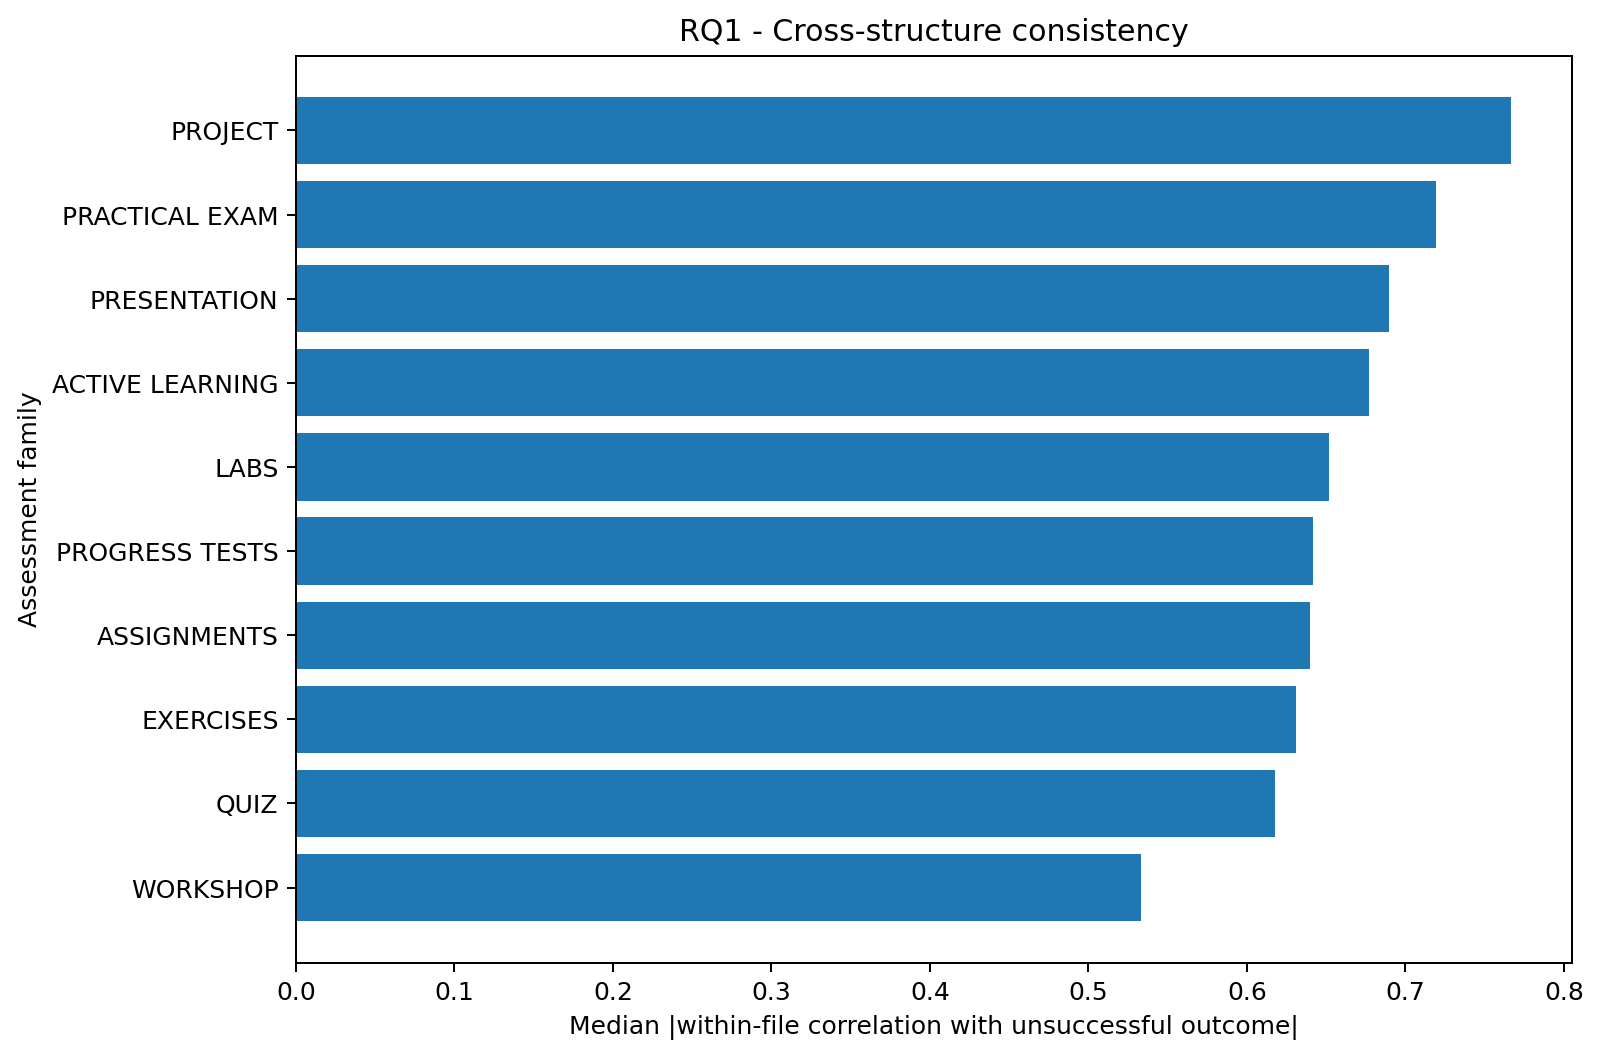
\includegraphics[height=.27\textheight,width=.68\textwidth,keepaspectratio]{figures/RQ1_cross_structure_consistency.png}
\caption{RQ1. Within-file median absolute Pearson association by family, including families with fewer than five sources. File coverage determines eligibility for the primary comparison.}
\label{fig:rq1}
\end{figure}



\subsection{RQ2. Random Forest leads on validation F2}
Table~\ref{tab:rq2} and Fig.~\ref{fig:rq2} show five candidate models compared at threshold 0.50 on 22,236 validation rows. Random Forest achieves the largest F2 (0.8566), 0.0091 ahead of LightGBM (0.8475), and the highest recall (0.8586). The three boosted models have higher precision (0.9449 to 0.9524) and higher PR-AUC (0.9444 to 0.9464) than Random Forest (0.8489 and 0.9309). The Decision Tree has the lowest precision and PR-AUC. The model ranks therefore depend on the chosen metric. The fitted Random Forest's test result at the same threshold, F2 0.8409, becomes the fixed-threshold baseline in RQ3.

\begin{table}[h]
\caption{RQ2 validation results for five tree classifiers and two reference methods.}
\label{tab:rq2}
\centering
\begin{tabular}{lrrrr}
\toprule
Model & F2 & Recall & Precision & PR-AUC \\
\midrule
Random Forest & 0.8566 & 0.8586 & 0.8489 & 0.9309 \\
LightGBM & 0.8475 & 0.8262 & 0.9449 & 0.9464 \\
XGBoost & 0.8459 & 0.8233 & 0.9503 & 0.9464 \\
CatBoost & 0.8386 & 0.8143 & 0.9524 & 0.9444 \\
Decision Tree & 0.8374 & 0.8438 & 0.8129 & 0.7835 \\
% CHECK: the logistic regression row is not produced by the v1.1 script. Recompute it with the
% v1.1 split and library versions, or confirm that the notebook value is still valid.
Logistic regression (L2) & 0.8248 & 0.8095 & 0.8922 & -- \\
Always flag & 0.6420 & 1.0000 & 0.2640 & -- \\
\bottomrule
\end{tabular}
\end{table}

\begin{figure}[h]
\centering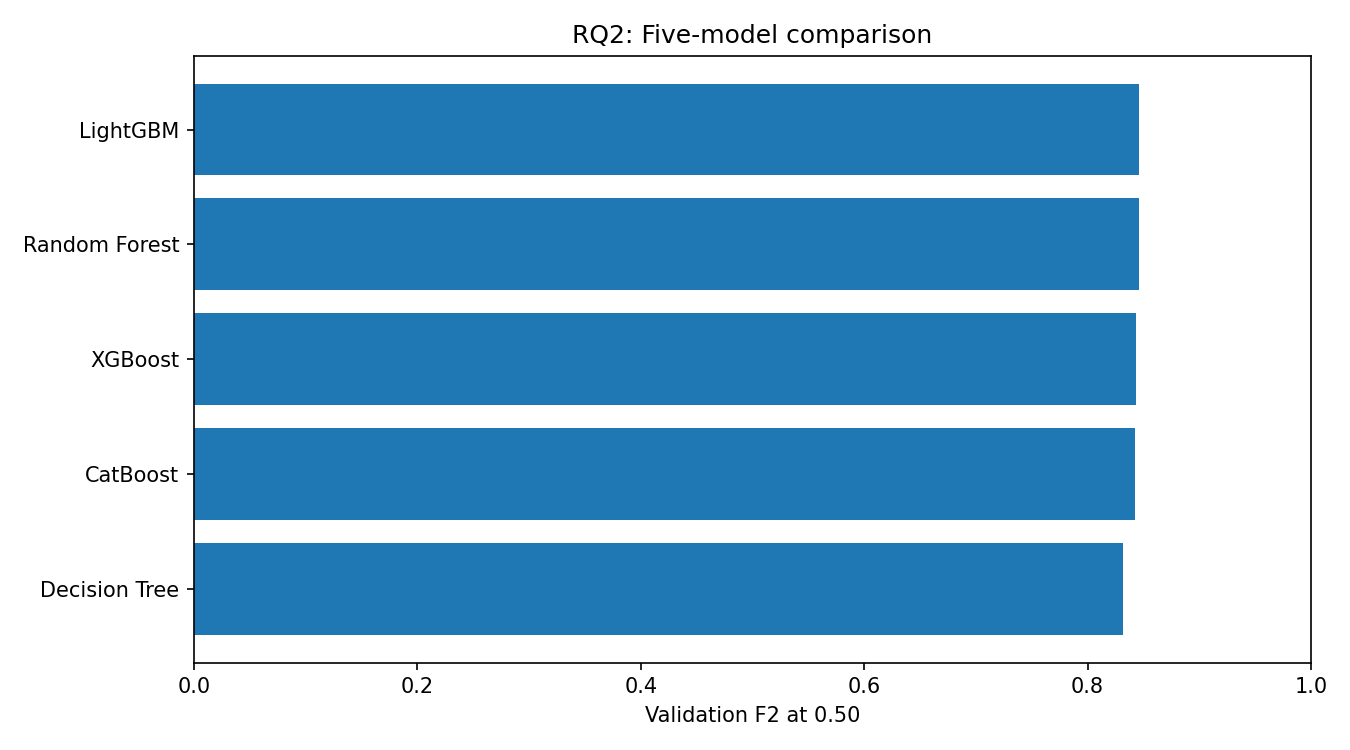
\includegraphics[width=.62\textwidth]{figures/RQ2_model_comparison.png}
\caption{RQ2. F2 for the five fitted candidates on validation at threshold 0.50. The two leading candidates, Random Forest and LightGBM, differ by approximately 0.0091.}
\label{fig:rq2}
\end{figure}

The always-flag rule has 5,870 true positives, 16,366 false positives, and F2 of 0.6420. An L2 logistic regression uses median imputation and standardization fitted on train, with the same 21 predictors and split. It gives F2 of 0.8248 at threshold 0.50. This contrast benchmarks a model with a linear log-odds assumption. A single split cannot establish whether the 0.0091 lead over LightGBM persists across terms.

\subsection{RQ3. SMOTE with tuning adds a small F2 gain through precision, not recall}
\begin{table}[h]
\caption{RQ3 test results on the same 21,977 attempts. Baseline and SMOTE use the Random Forest model family. The baseline uses raw inputs with missing values kept. The SMOTE rows and the imputed control (no SMOTE) use median-imputed inputs.}
\label{tab:rq3}
\centering
\setlength{\tabcolsep}{3pt}
\begin{tabular}{lrrrrrr}
\toprule
Scenario & Threshold & F2 & Recall & Precision & TP & FP \\
\midrule
Baseline, fixed & 0.50 & 0.8409 & 0.8399 & 0.8447 & 4,780 & 879 \\
Baseline, tuned & 0.39 & 0.8403 & 0.8593 & 0.7721 & 4,890 & 1,443 \\
SMOTE, fixed & 0.50 & 0.8356 & 0.8266 & 0.8739 & 4,704 & 679 \\
SMOTE, tuned & 0.34 & 0.8433 & 0.8563 & 0.7949 & 4,873 & 1,257 \\
\midrule
Control, fixed & 0.50 & 0.8406 & 0.8392 & 0.8461 & 4,776 & 869 \\
Control, tuned & 0.35 & 0.8408 & 0.8677 & 0.7481 & 4,938 & 1,663 \\
\bottomrule
\end{tabular}
\end{table}

\begin{figure}[h]
\centering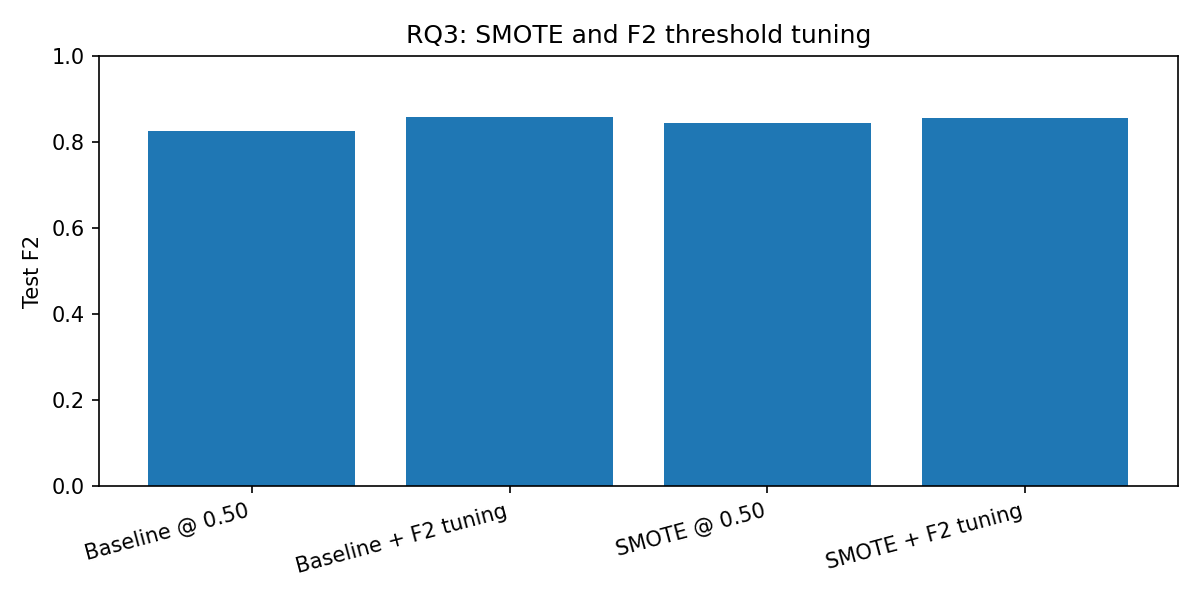
\includegraphics[width=.72\textwidth]{figures/RQ3_four_scenarios.png}
\caption{RQ3. F2 across fixed and tuned Random Forest operating points on the test partition. Recall and precision appear in Table~\ref{tab:rq3}.}
\label{fig:rq3}
\end{figure}

At a fixed threshold of 0.50, SMOTE lowers F2 from 0.8409 to 0.8356 and recall from 0.8399 to 0.8266. After each variant receives a validation-selected threshold, the tuned SMOTE model is ahead in F2 by 0.0030 (0.8433 against 0.8403) and in precision by 0.0228, but its recall is 0.0030 lower. Tuning the baseline alone raises recall by 0.0193 and leaves F2 essentially unchanged ($-0.0006$): it finds 110 more unsuccessful attempts at the cost of 564 more false warnings. Imputation alone changes baseline F2 by only $-0.0003$ at threshold 0.50. Against the imputed control, tuned SMOTE adds 0.0025 F2 and 0.0469 precision and loses 0.0114 recall. SMOTE therefore does not improve recall here. Its small F2 gain comes from fewer false warnings.

\section{Discussion and Limitations}
\subsection{Interpreting the screening trade-off}
The findings support three separate decisions. RQ1 identifies Practical Exam as a promising descriptive signal when coverage across source files matters. RQ2 selects Random Forest under the designated validation rule. RQ3 finds a small F2 advantage for the tuned SMOTE variant, obtained through higher precision and a smaller review queue, while the tuned baseline keeps slightly higher recall.

The test cohort contains 5,691 unsuccessful and 16,286 successful attempts. At the tuned baseline threshold, the review queue contains 6,333 attempts, of which 4,890 are true positives. The tuned SMOTE queue contains 6,130 attempts, of which 4,873 are true positives. The 203 extra reviews of the baseline consist of 17 additional detections and 186 additional warnings for attempts that eventually passed. These counts describe observed errors under historical outcomes. The eventual costs and benefits of intervention depend on staff capacity, timing and the form of support.

\subsection{Validity and generalization}
\textbf{Assessment availability.} The exclusion of Final Exam and TOTAL respects the intended feature window. A component called Practical Exam can occur late in a term, so scheduled grade publication needs independent verification before live use.

\textbf{Coverage and missingness.} The analysis conditions on a usable score for modeling and on complete score--label pairs for RQ1. Missing scores can be structural. Results therefore characterize the eligible population and do not describe all cleaned records or every assessment format.

\textbf{Repeated records.} The 4,812 repeated keys (9,625 rows) remain in all analyses while they are under review. If some are duplicate entries, training rows and RQ1 score--label pairs are partly redundant, and the reported correlations and metrics could shift slightly after deduplication.

\textbf{Identity and time.} A file-scoped code prevents overlap for the composite key. The current split does not hold out whole terms or prove that equivalent identities across source files are independent. A temporal holdout would measure whether the selected threshold travels to a new offering.

\textbf{Run sensitivity.} The RQ2 margin (0.0091 over LightGBM) and the tuned RQ3 differences (0.0030 in F2 and in recall) are descriptive. No paired uncertainty interval is reported. An earlier archived run, with median-imputed inputs for all models and older library versions, ranked LightGBM first by 0.0006 over Random Forest. The artifacts do not isolate whether imputation or library versions produced the change, so the model ranking should not be treated as stable.

\textbf{Deployment and causal claims.} The outcome merges academic non-passing with attendance failure. It does not directly measure why an attempt was unsuccessful. A historical F2 score measures screening quality, while a prospective study would be required to evaluate benefits of a support program.

\section{Conclusion and Future Work}
Practical Exam showed the strongest median absolute association among families represented in at least five files ($|r|=0.7193$ across ten sources). Random Forest ranked first among five candidates by validation F2 (0.8566). The same model family without SMOTE achieved test F2 of 0.8403 at its tuned threshold, compared with 0.8433 for the tuned SMOTE variant. The tuned baseline keeps slightly higher recall (0.8593 against 0.8563) and incurs more false warnings, so the SMOTE gain is small and does not come from recall. The dashboard displays these results alongside the underlying coverage and decision counts.

For a follow-up evaluation, a new-term holdout and grade release timestamps would establish how early the system could issue actionable flags and how performance changes over time. Paired uncertainty estimates would help quantify how much model or threshold differences vary. An intervention study would address whether review leads to beneficial student outcomes.

\begin{thebibliography}{9}
\bibitem{arnold} Arnold, K.E., Pistilli, M.D.: Course signals at Purdue: Using learning analytics to increase student success. In: Proc. LAK, pp. 267--270 (2012). \href{https://doi.org/10.1145/2330601.2330666}{doi:10.1145/2330601.2330666}
\bibitem{jaya} Jayaprakash, S.M., Moody, E.W., Laur\'ia, E.J.M., Regan, J.R., Baron, J.D.: Early alert of academically at-risk students: An open source analytics initiative. J. Learn. Anal. 1(1), 6--47 (2014). \href{https://doi.org/10.18608/jla.2014.11.3}{doi:10.18608/jla.2014.11.3}
\bibitem{breiman} Breiman, L.: Random forests. Mach. Learn. 45, 5--32 (2001). \href{https://doi.org/10.1023/A:1010933404324}{doi:10.1023/A:1010933404324}
\bibitem{chen} Chen, T., Guestrin, C.: XGBoost: A scalable tree boosting system. In: Proc. KDD, pp. 785--794 (2016). \href{https://doi.org/10.1145/2939672.2939785}{doi:10.1145/2939672.2939785}
\bibitem{ke} Ke, G., et al.: LightGBM: A highly efficient gradient boosting decision tree. In: Advances in Neural Information Processing Systems 30 (2017).
\bibitem{cat} Prokhorenkova, L., et al.: CatBoost: Unbiased boosting with categorical features. In: Advances in Neural Information Processing Systems 31 (2018).
\bibitem{fbeta} Scikit-learn developers: F-beta score. \url{https://scikit-learn.org/stable/modules/generated/sklearn.metrics.fbeta_score.html}
\bibitem{smote} Chawla, N.V., Bowyer, K.W., Hall, L.O., Kegelmeyer, W.P.: SMOTE: Synthetic minority over-sampling technique. J. Artif. Intell. Res. 16, 321--357 (2002). \href{https://doi.org/10.1613/jair.953}{doi:10.1613/jair.953}
\end{thebibliography}
\end{document}
